
\section{Existing games}

	\subsection{Parallel Kingdom}
	The game was developed by PerBlue and released in October 2008. Parallel Kingdom is the most similar game to ours.
		
	\textit{"Parallel Kingdom is a mobile, location based, massively multiplayer game that uses GPS location and Google Maps to place users in a virtual world. Parallel Kingdom is the first location based RPG for the iOS and Android platforms. The game is set in a virtual world or ”Parallel Kingdom” where users claim their territories based on their GPS location or by making friends who invite them to travel to new places."} \cite{parallelkingdom}
	
	The game gained on popularity and even reached 1 million player by the end of January 2012 \cite{parallelkingdom1m}. Parallel Kingdom discontinued on November 1, 2016 for undisclosed reasons.
	
	\begin{figure}[h]	
		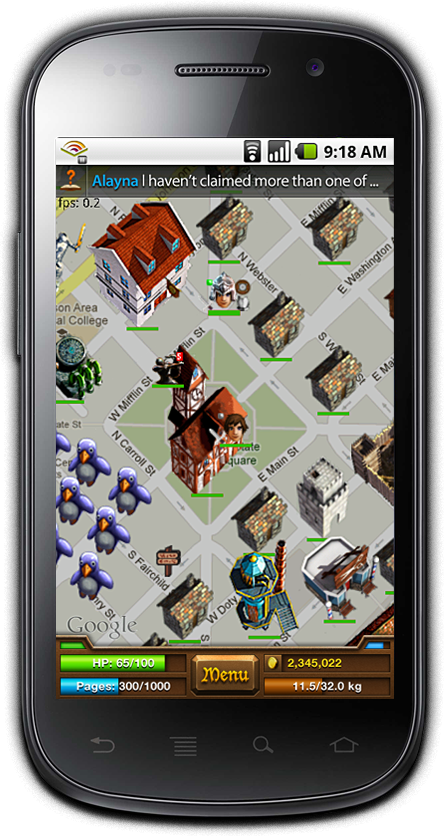
\includegraphics[width=0.33\textwidth]{figures/parallelkingdom}
		\centering			
		\caption{Screenshot of Parallel Kingdom \cite{parallelkingdomscreen}}
	\end{figure}
	
	\subsection{Ingress}
	Developed by Niantic, which was then part of Google, the game was released in December 2013 for Android, followed by an iOS version in June 2014. It is a location based, massively multiplayer game. A player joins one of two factions, Enlightened or Resistance, and then as a part of his team capture regions of the game map. Fate of the factions relies on players’ cooperation. Thanks to that players meet in real life and coordinate their actions.
	
	\textit{"Move through the real world using your Android device and the Ingress app to discover and tap sources of this mysterious energy. Acquire objects to aid in your quest, deploy tech to capture territory, and ally with other players to advance the cause of the Enlightened or the Resistance."} \cite{ingress}
	
	Ingress is a very successful augmented reality game with tens of millions installs.
	
	\subsection{Pokémon GO}
	After its success with Ingress, Niantic started working on a new game Pokemon GO. Released in July 2016, the game became an incredible hit. Even though the game faced many problems during its launch, mainly caused by the unexpected success and more active users than Pokémon	GO servers were able to handle, in the first 80 days Pokémon GO reached about 550 millions downloads and earned about \$470 million \cite{pokemongosuccess}.
	
	\textit{"Venusaur, Charizard, Blastoise, Pikachu, and many other Pokémon have been discovered! Now’s your chance to discover and capture the Pokémon all around you—so get your shoes on, step outside, and explore the world. You’ll join one of three teams and battle for the prestige and ownership of Gyms with your Pokémon at your side."} \cite{pokemongo}
		
	Pokémon GO is very similar to Ingress and uses the same crowd-sourced geographical data.
	
\section{Use Cases}
	\subsection{Actors}
		\begin{figure}[h]	
			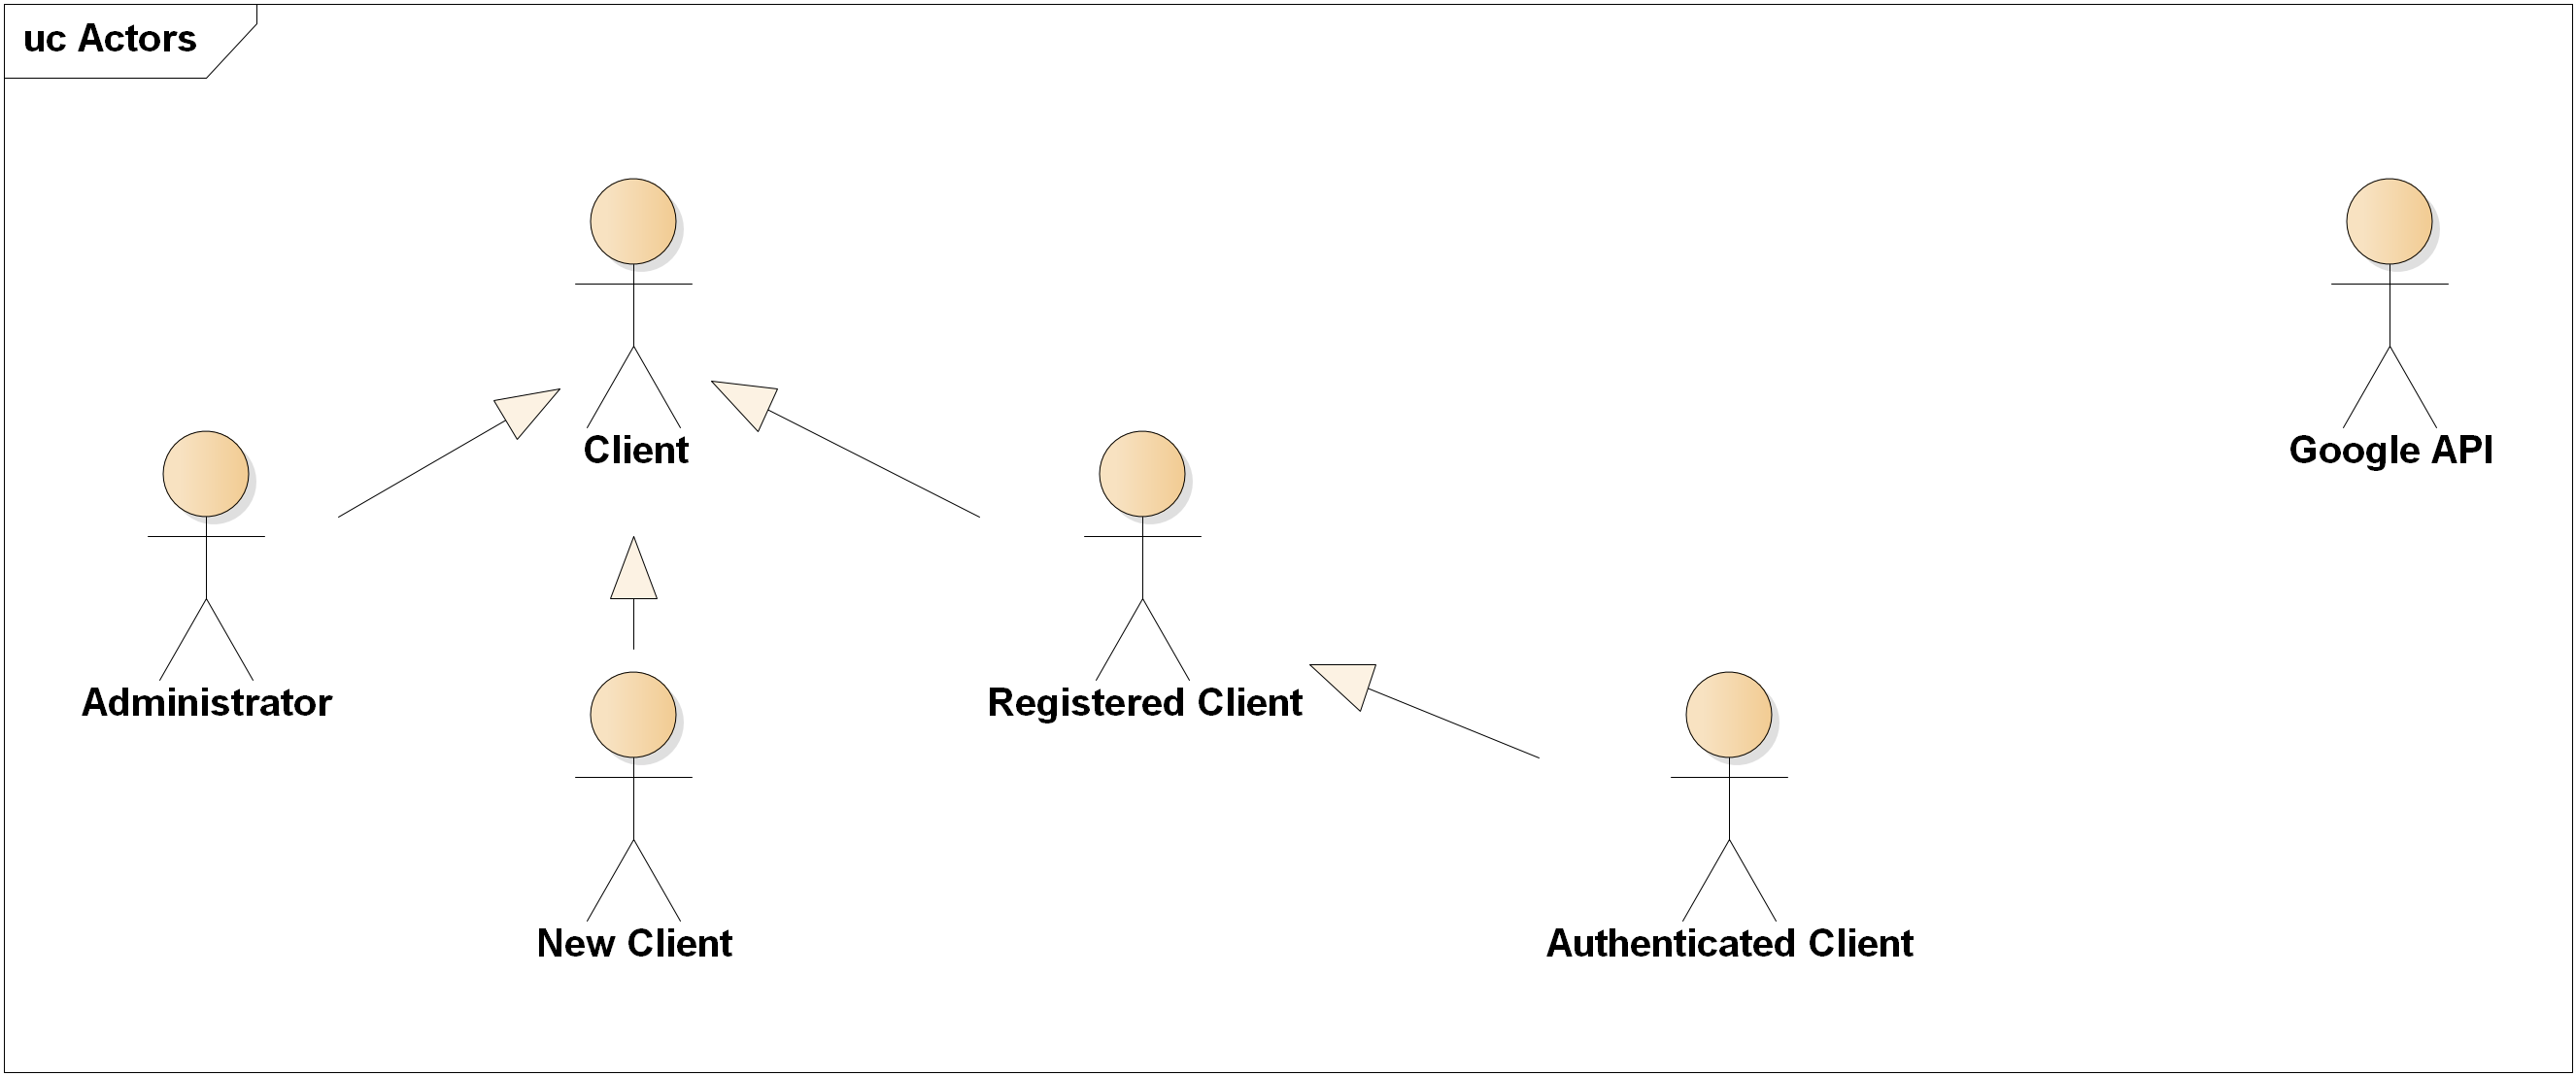
\includegraphics[width=\textwidth]{figures/UC_Actors}
			\centering			
			\caption{Use Case
				 Diagram -- Actors}
			\label{fig:ucactors}
		\end{figure}
		\noindent Actor is a role played by a user or other system that interacts with the server. The most general role is \textit{Client} and anyone who accesses the server through API is considered to play either this role or any of its children. From now on, the terms client and user will be used interchangeably. Refer to Figure \ref{fig:ucactors} for the role hierarchy.
		
		\textit{Administrator} is a client who has privilege to create and maintain the functionality of the game. \textit{New Client} is a user who is not yet registered and probably accesses the game for the first time. \textit{Registered Client} is the default role for a user who already has a valid account but is not logged in. Lastly, \textit{Authenticated Client} has all the required privileges to play the game. This client will be refereed to as \textit{player}. The last main actor is Google API which provides the access to Google services. 		

	\subsection{Authentication}	
	\begin{figure}[h]	
		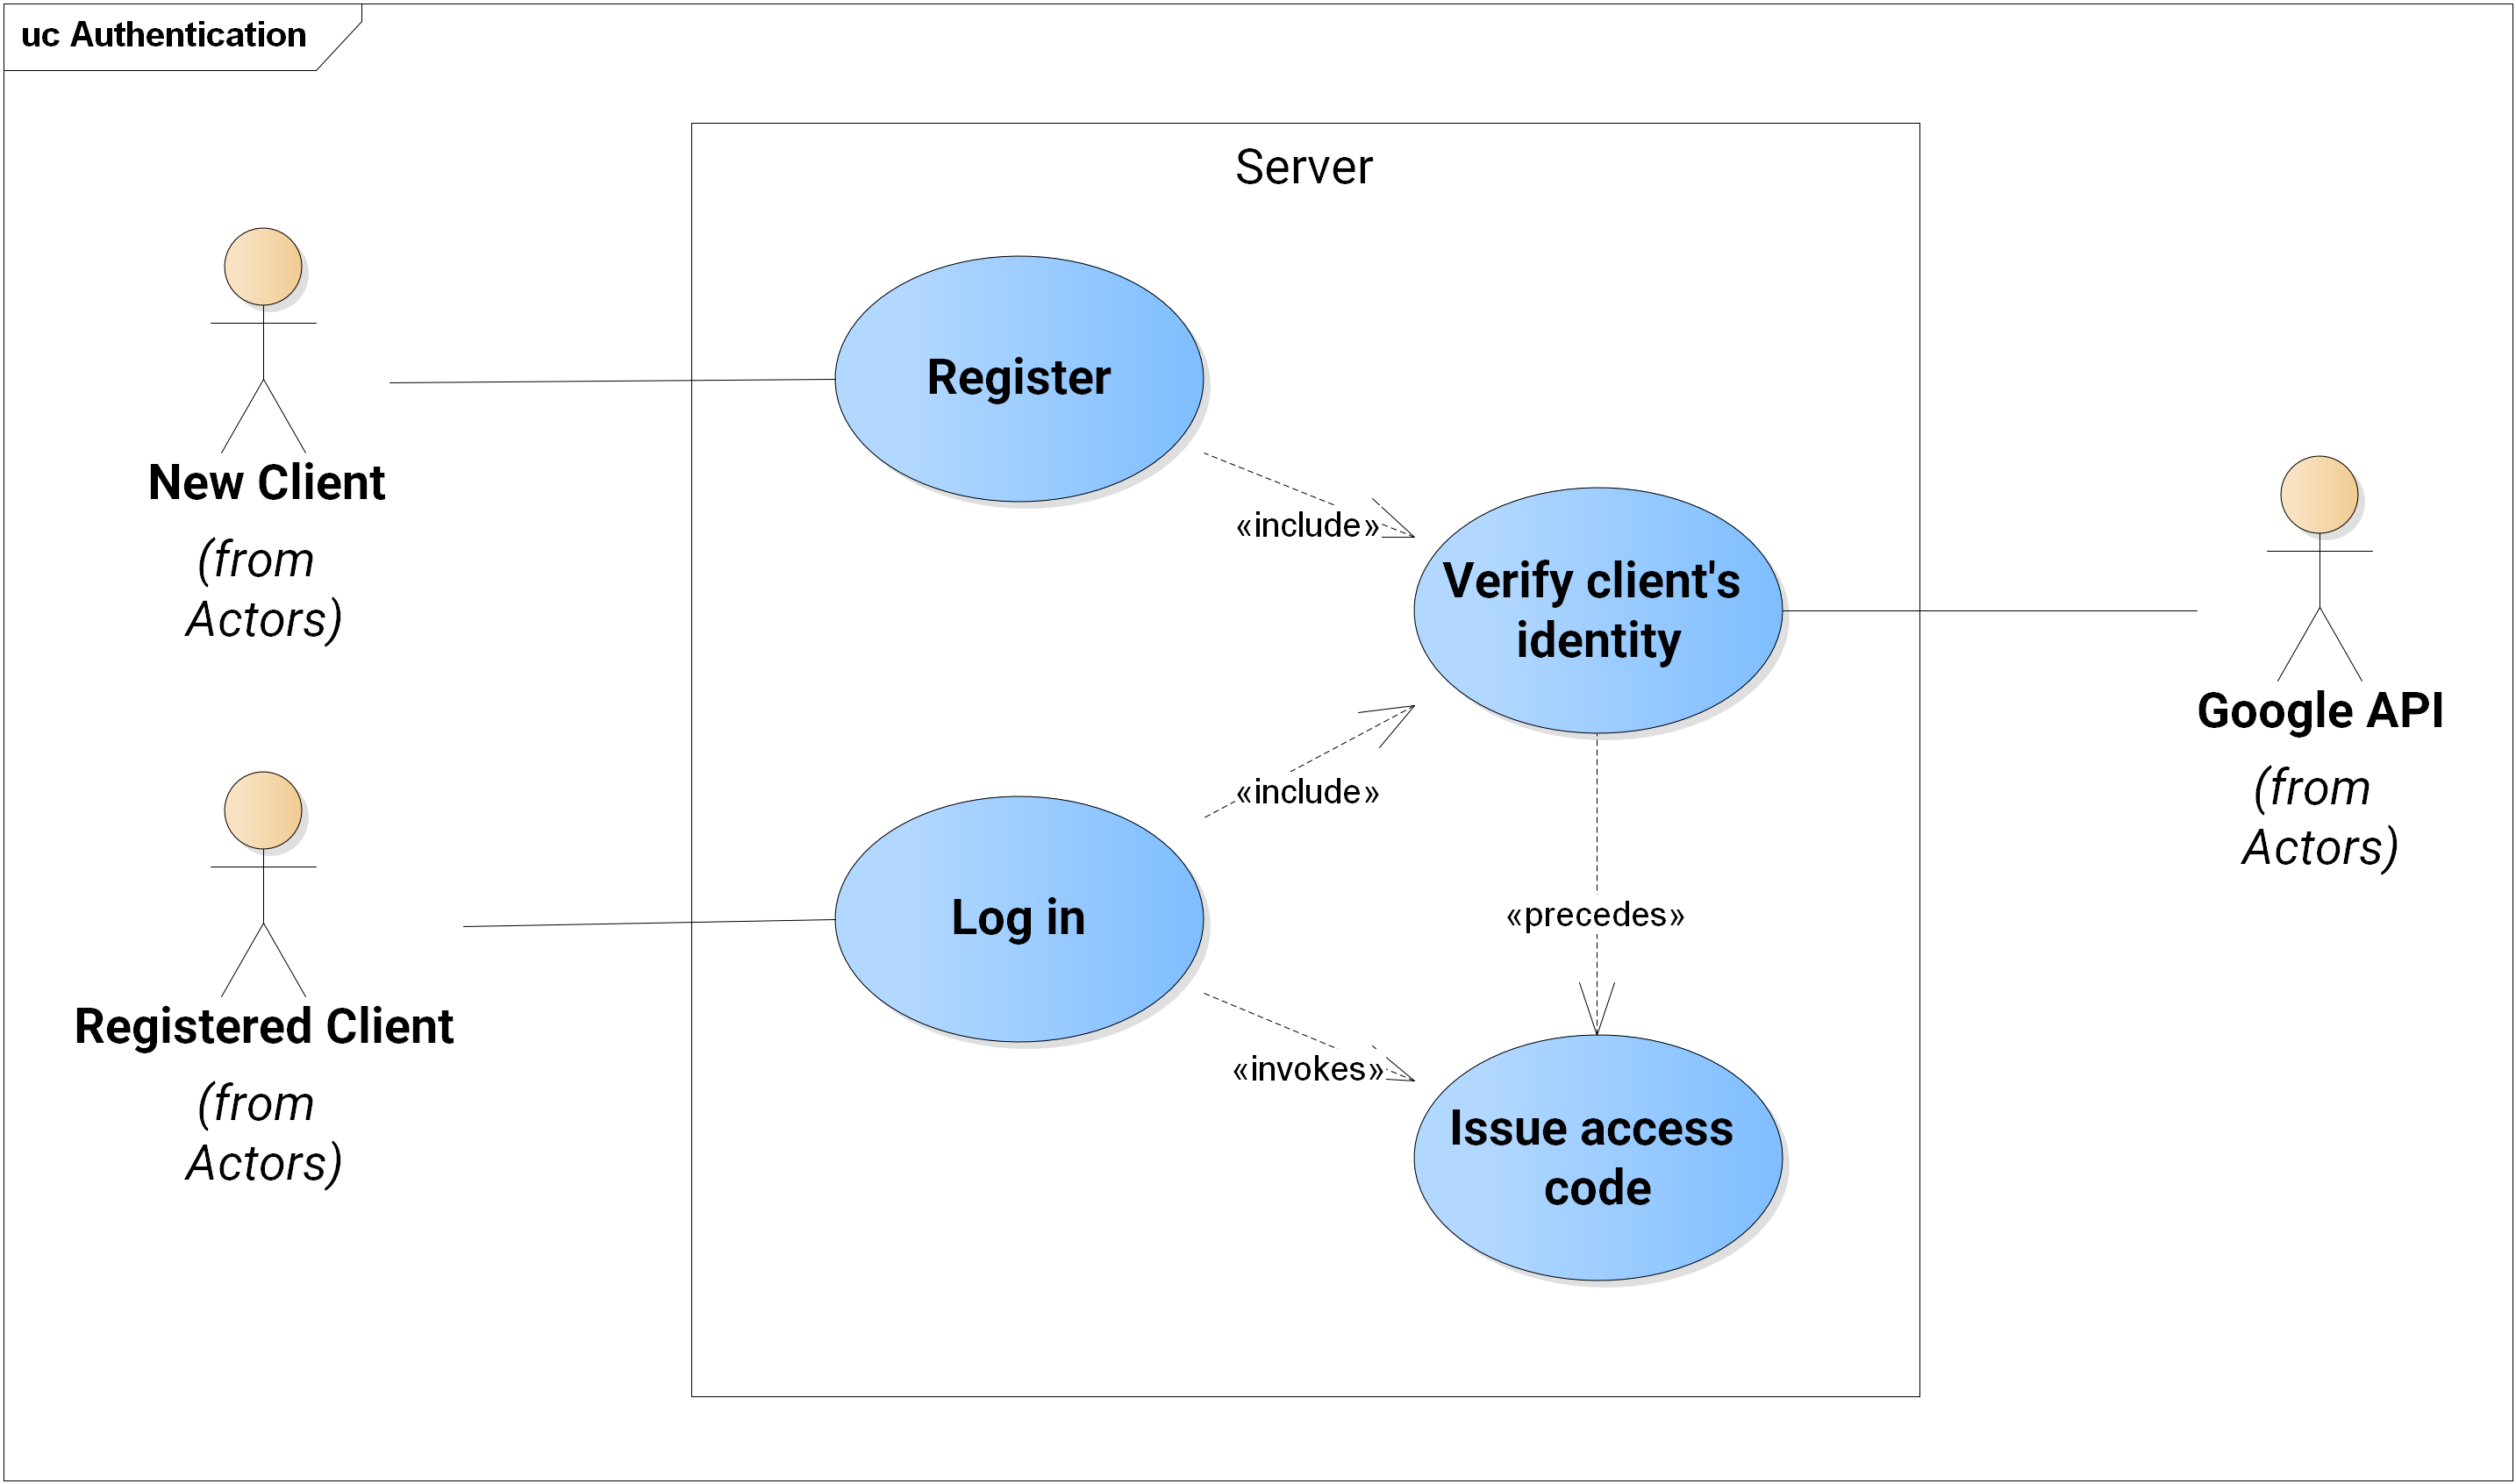
\includegraphics[width=\textwidth]{figures/UC_Authentication}
		\centering			
		\caption{Use Case Diagram -- Client's authentication}
		\label{fig:ucauth}
	\end{figure}
	\noindent Authentication use cases user performs to get promoted to more privileged roles. The basic transition flow is \textit{New Client} $\rightarrow$ \textit{Registered Client} $\rightarrow$ \textit{Authenticated Client}. See Figure \ref{fig:ucauth}.
	
	\begin{itemize}
		\item \textbf{Register} \\
		The only choice \textit{New Client} has is to register a new account. He uses provides his Google identity and chooses an username. After his identity is verified, the server creates a new profile and logs the user in.
		
		\item \textbf{Log in} \\
		The \textit{Registered Client} must log in before he can access any of the game features. He provides his Google identity which is then verified and matched to an account. An access code is issued for the future identification within the session.		
		
		\item \textbf{Verify user's identity} \\
		Proper verification is needed when the game server receives a Google identity of a user. The server contacts the \textit{Google API} which responds with user's personal information if the identity is valid.
		
		\item \textbf{Issue access code} \\ 
		This use case is invoked during login process. Server issues a unique access code to the user. Only \textit{Authenticated Client} has such code.
	\end{itemize}
	
	\subsection{Actions}	
		\begin{figure}[h]	
			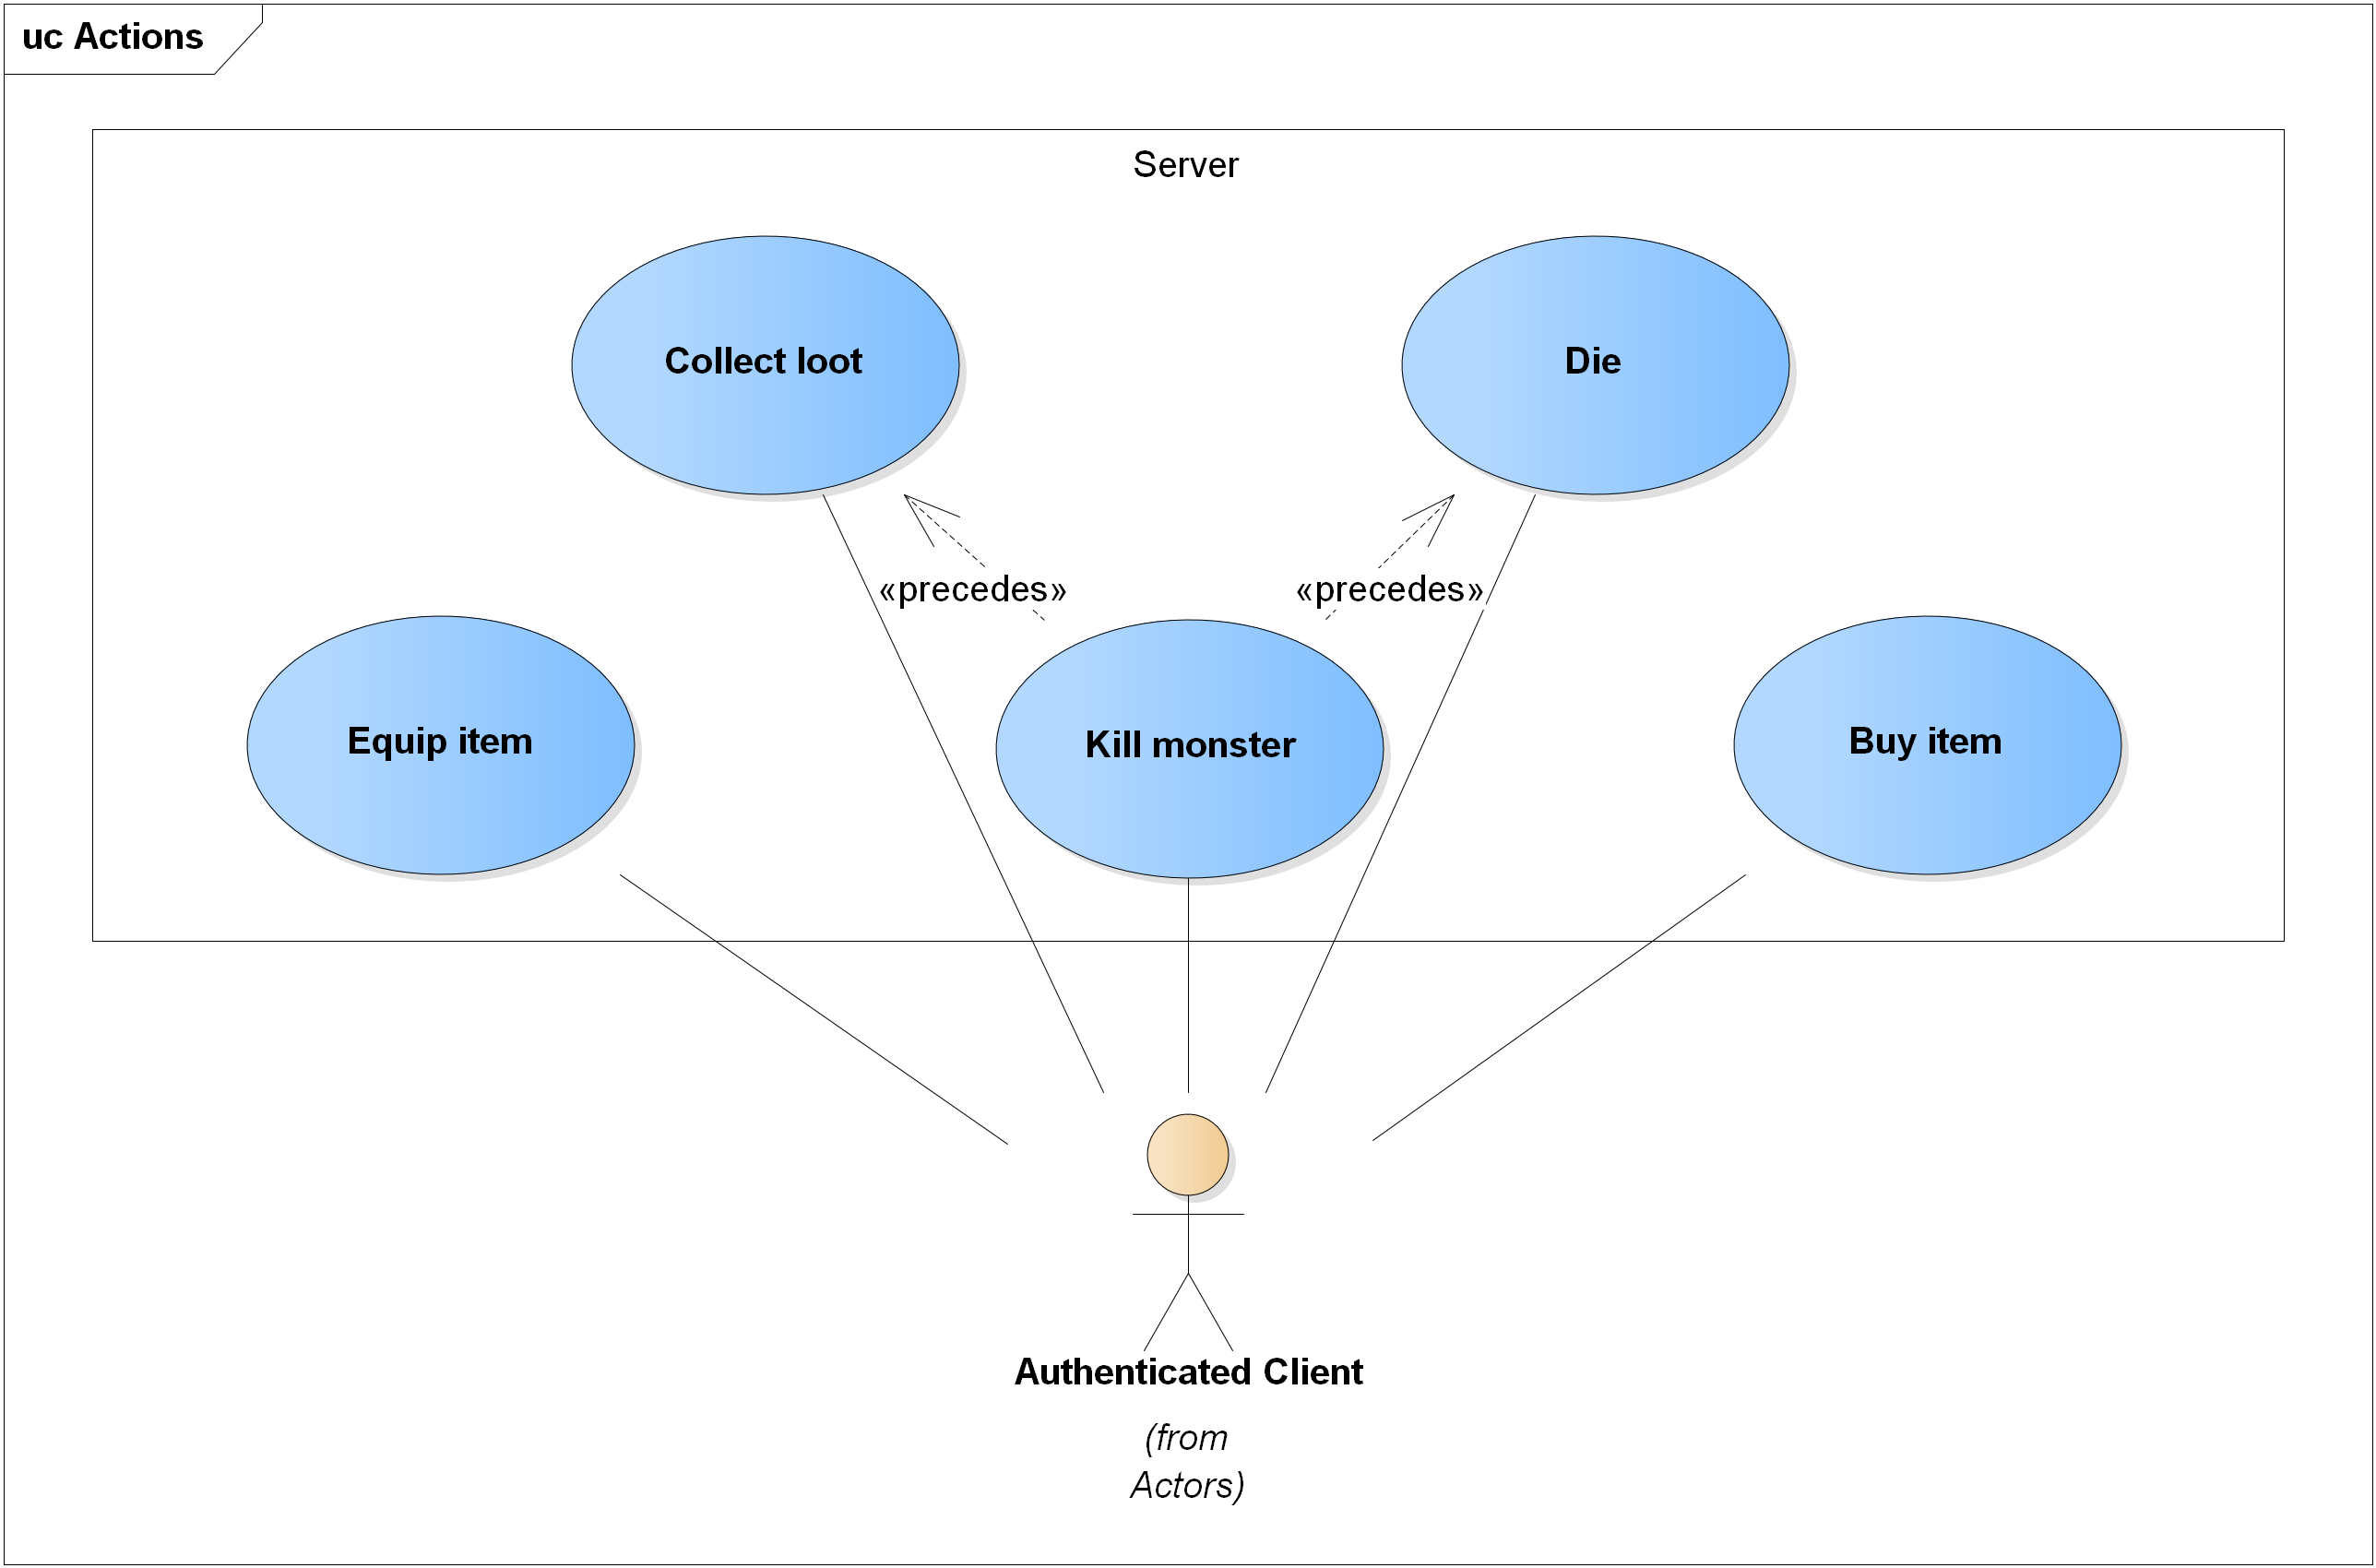
\includegraphics[width=\textwidth]{figures/UC_Actions}
			\centering			
			\caption{Use Case Diagram -- Player's actions}
			\label{fig:ucactions}
		\end{figure}
		\noindent Action is an event triggered by player's interaction with a game object. See the diagram in Figure \ref{fig:ucactions}.
		
		\begin{itemize}
			\item \textbf{Equip item} \\
			A player wants to equip an item from his inventory. The item will be assigned to a specific slot. For example the player equips a sword to his right hand.
			
			\item \textbf{Buy item} \\
			A player wants to exchange gold in a shop for an item he chooses. When the purchase is finished, the player receives the item to his inventory.
			
			\item \textbf{Kill monster} \\
			A player wants to kill monsters to progress in the game. If he successfully kills the monster, he is rewarded with gold and experience
			
			\item \textbf{Collect loot} \\
			This action must be preceded by the \textit{Kill monster} use case. A player can choose to collect loot from the monster he killed.
			
			\item \textbf{Die} \\
			This action must be preceded by the \textit{Kill monster} use case. A player who lost his fight against a monster dies and is punished with some penalty.		
		\end{itemize}
	
	\subsection{Miscellaneous}
	\begin{figure}[h]	
		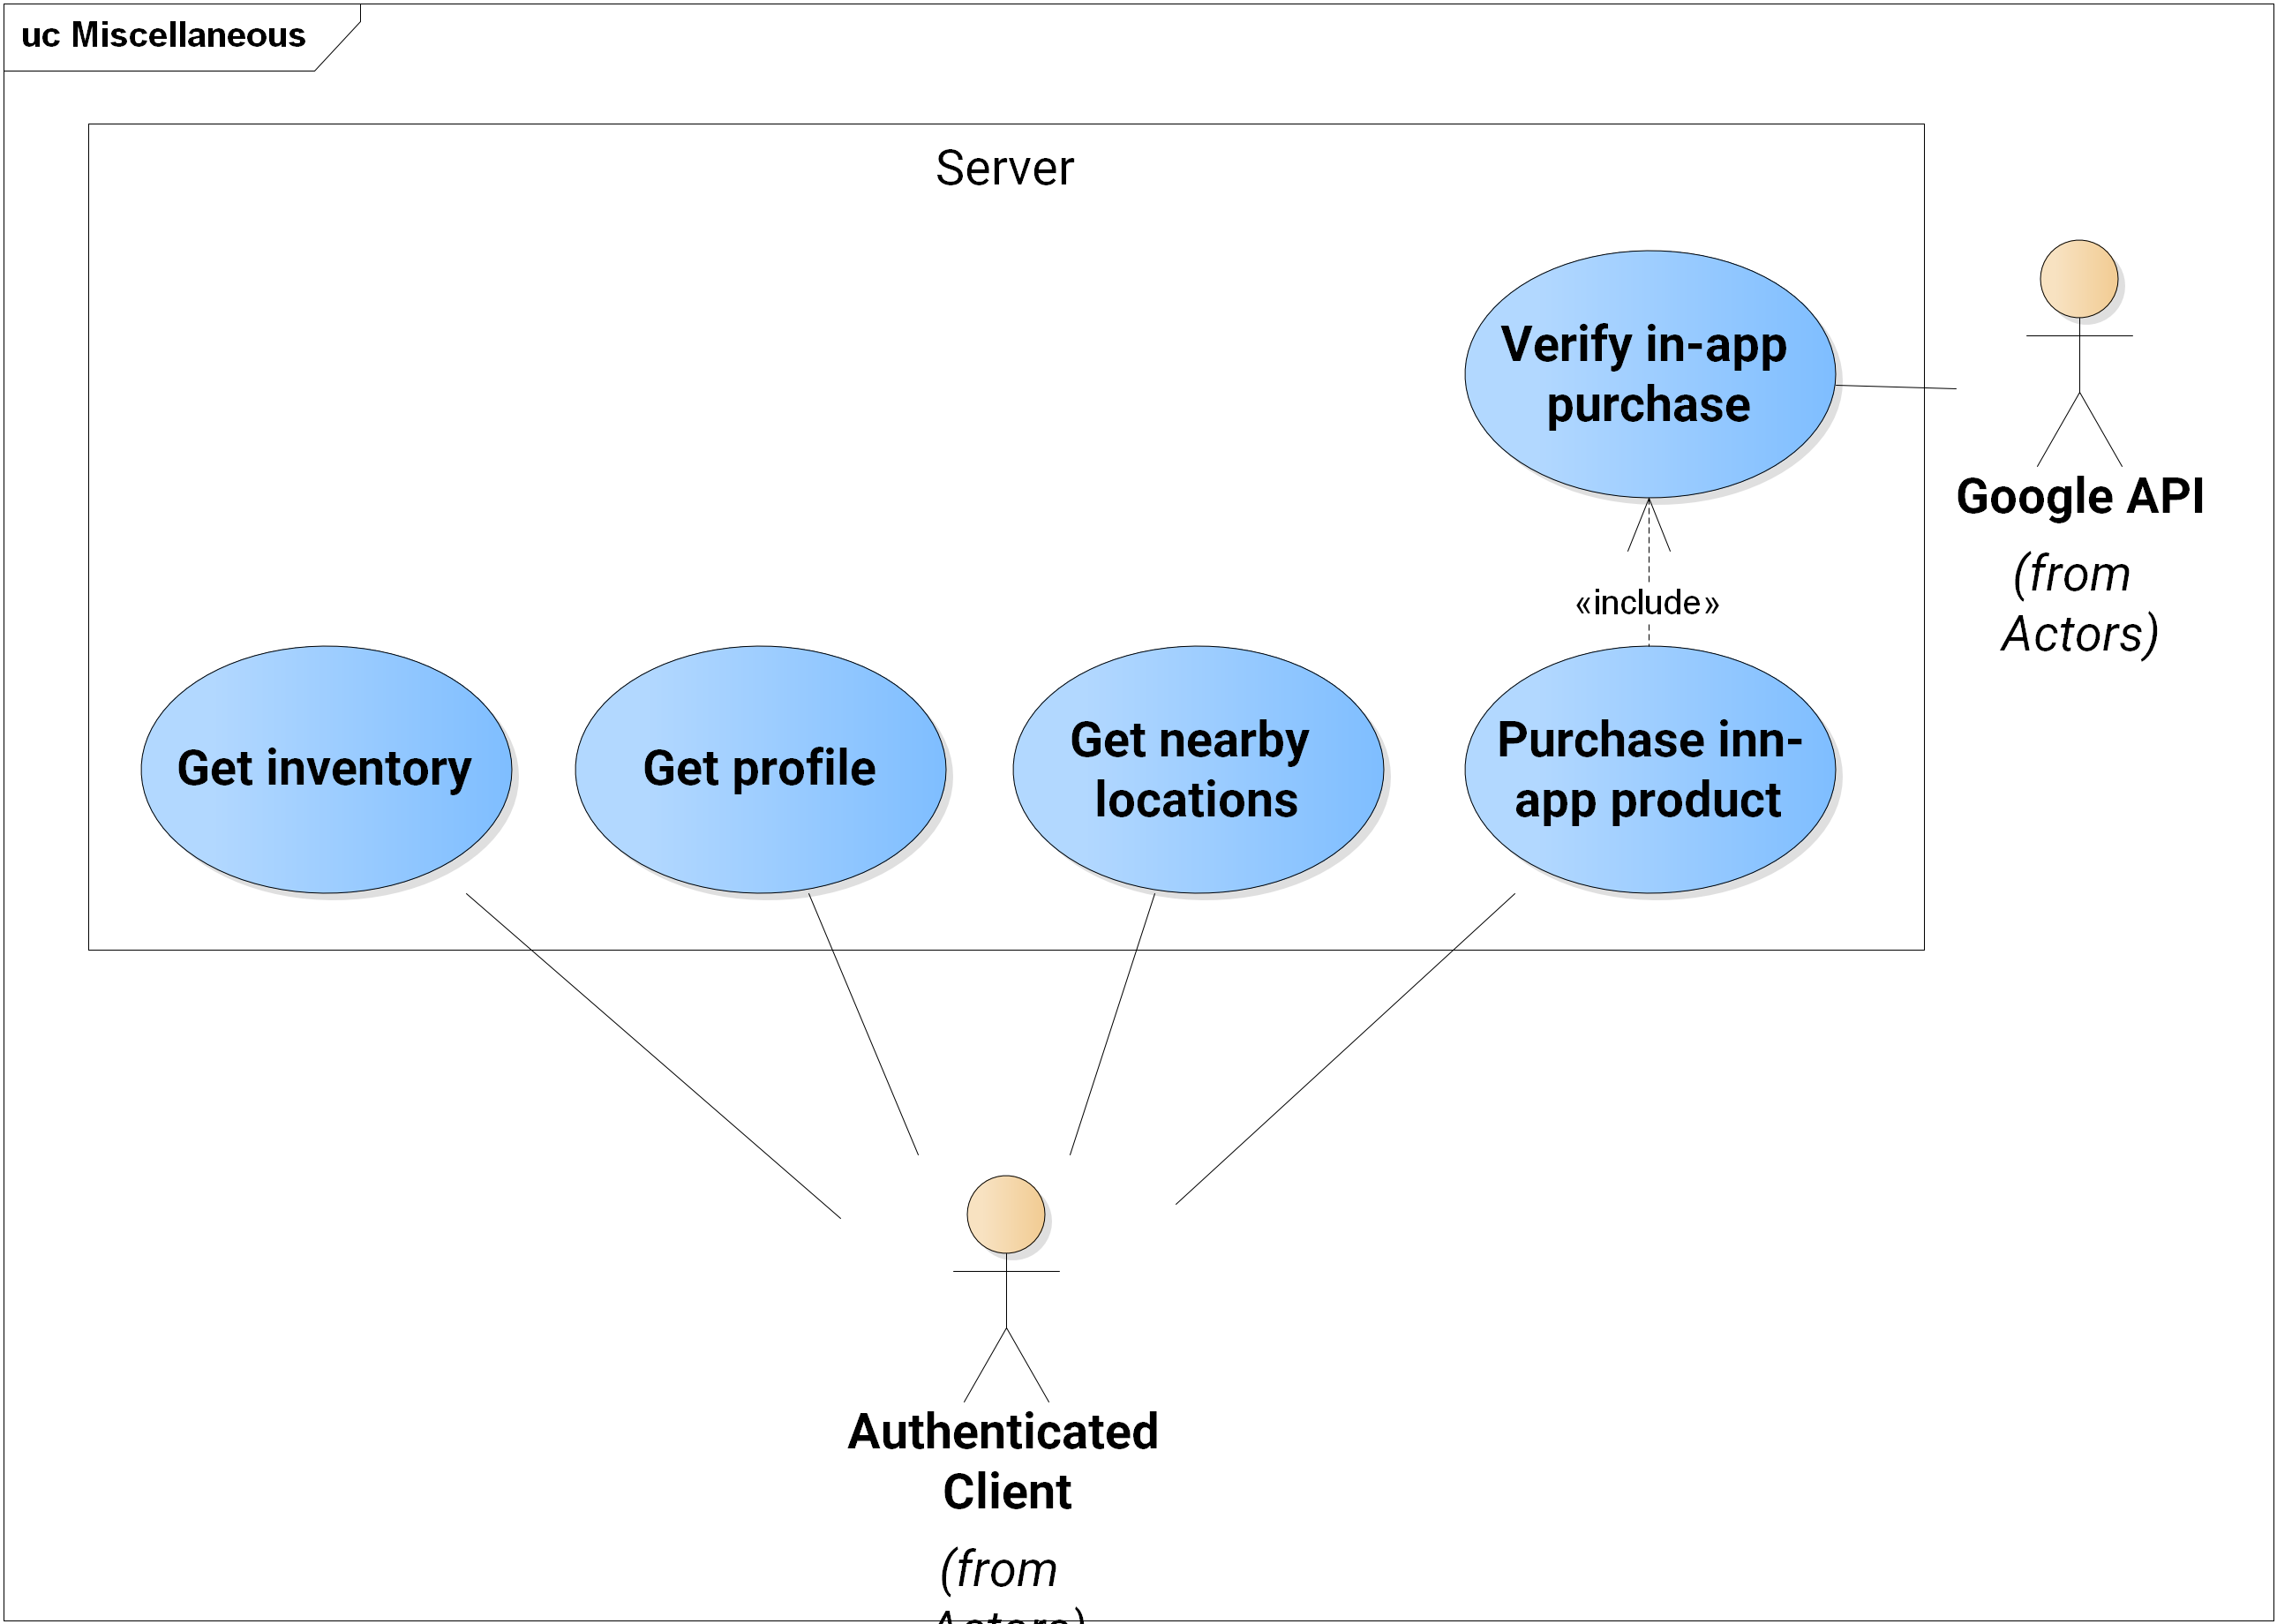
\includegraphics[width=\textwidth]{figures/UC_Miscellaneous}
		\centering			
		\caption{Use Cases: Miscellaneous}
		\label{fig:ucmisc}
	\end{figure}
	The following use cases mainly cover requests made by client application. See the diagram in Figure \ref{fig:ucmisc}.
	\begin{itemize}
		\item \textbf{Get inventory}\\
		The application requests all items the player owns. It is also possible to retrieve all the player's equipment with each item assigned to some slot.
		
		\item \textbf{Get profile}\\
		A client may need to synchronize its internal state of the players profile with the server. The application is provided with complete state of the player's profile including attributes like health, gold, and experience.
		
		
		\item \textbf{Get nearby locations}\\
		This is a critical functionality of the server. A client asks for game locations near his coordinates. The server provides such locations along with their associated game objects.
		
		
		\item \textbf{Purchase in-app product}\\
		The application supports micro-transactions. Since the purchase is made client-side, the application has to notify the server about the purchase and give the bought product to the player. 
		
		
		\item \textbf{Verify in-app purchase}\\
		During the previous use case (\textit{Purchase in-app product}), the server verifies if the purchase is valid and not fake, canceled, or already accounted. The verification process is done through \textit{Google API}.
		
		
	\end{itemize}
	

	\subsection{Administration}
	\begin{figure}[h]	
		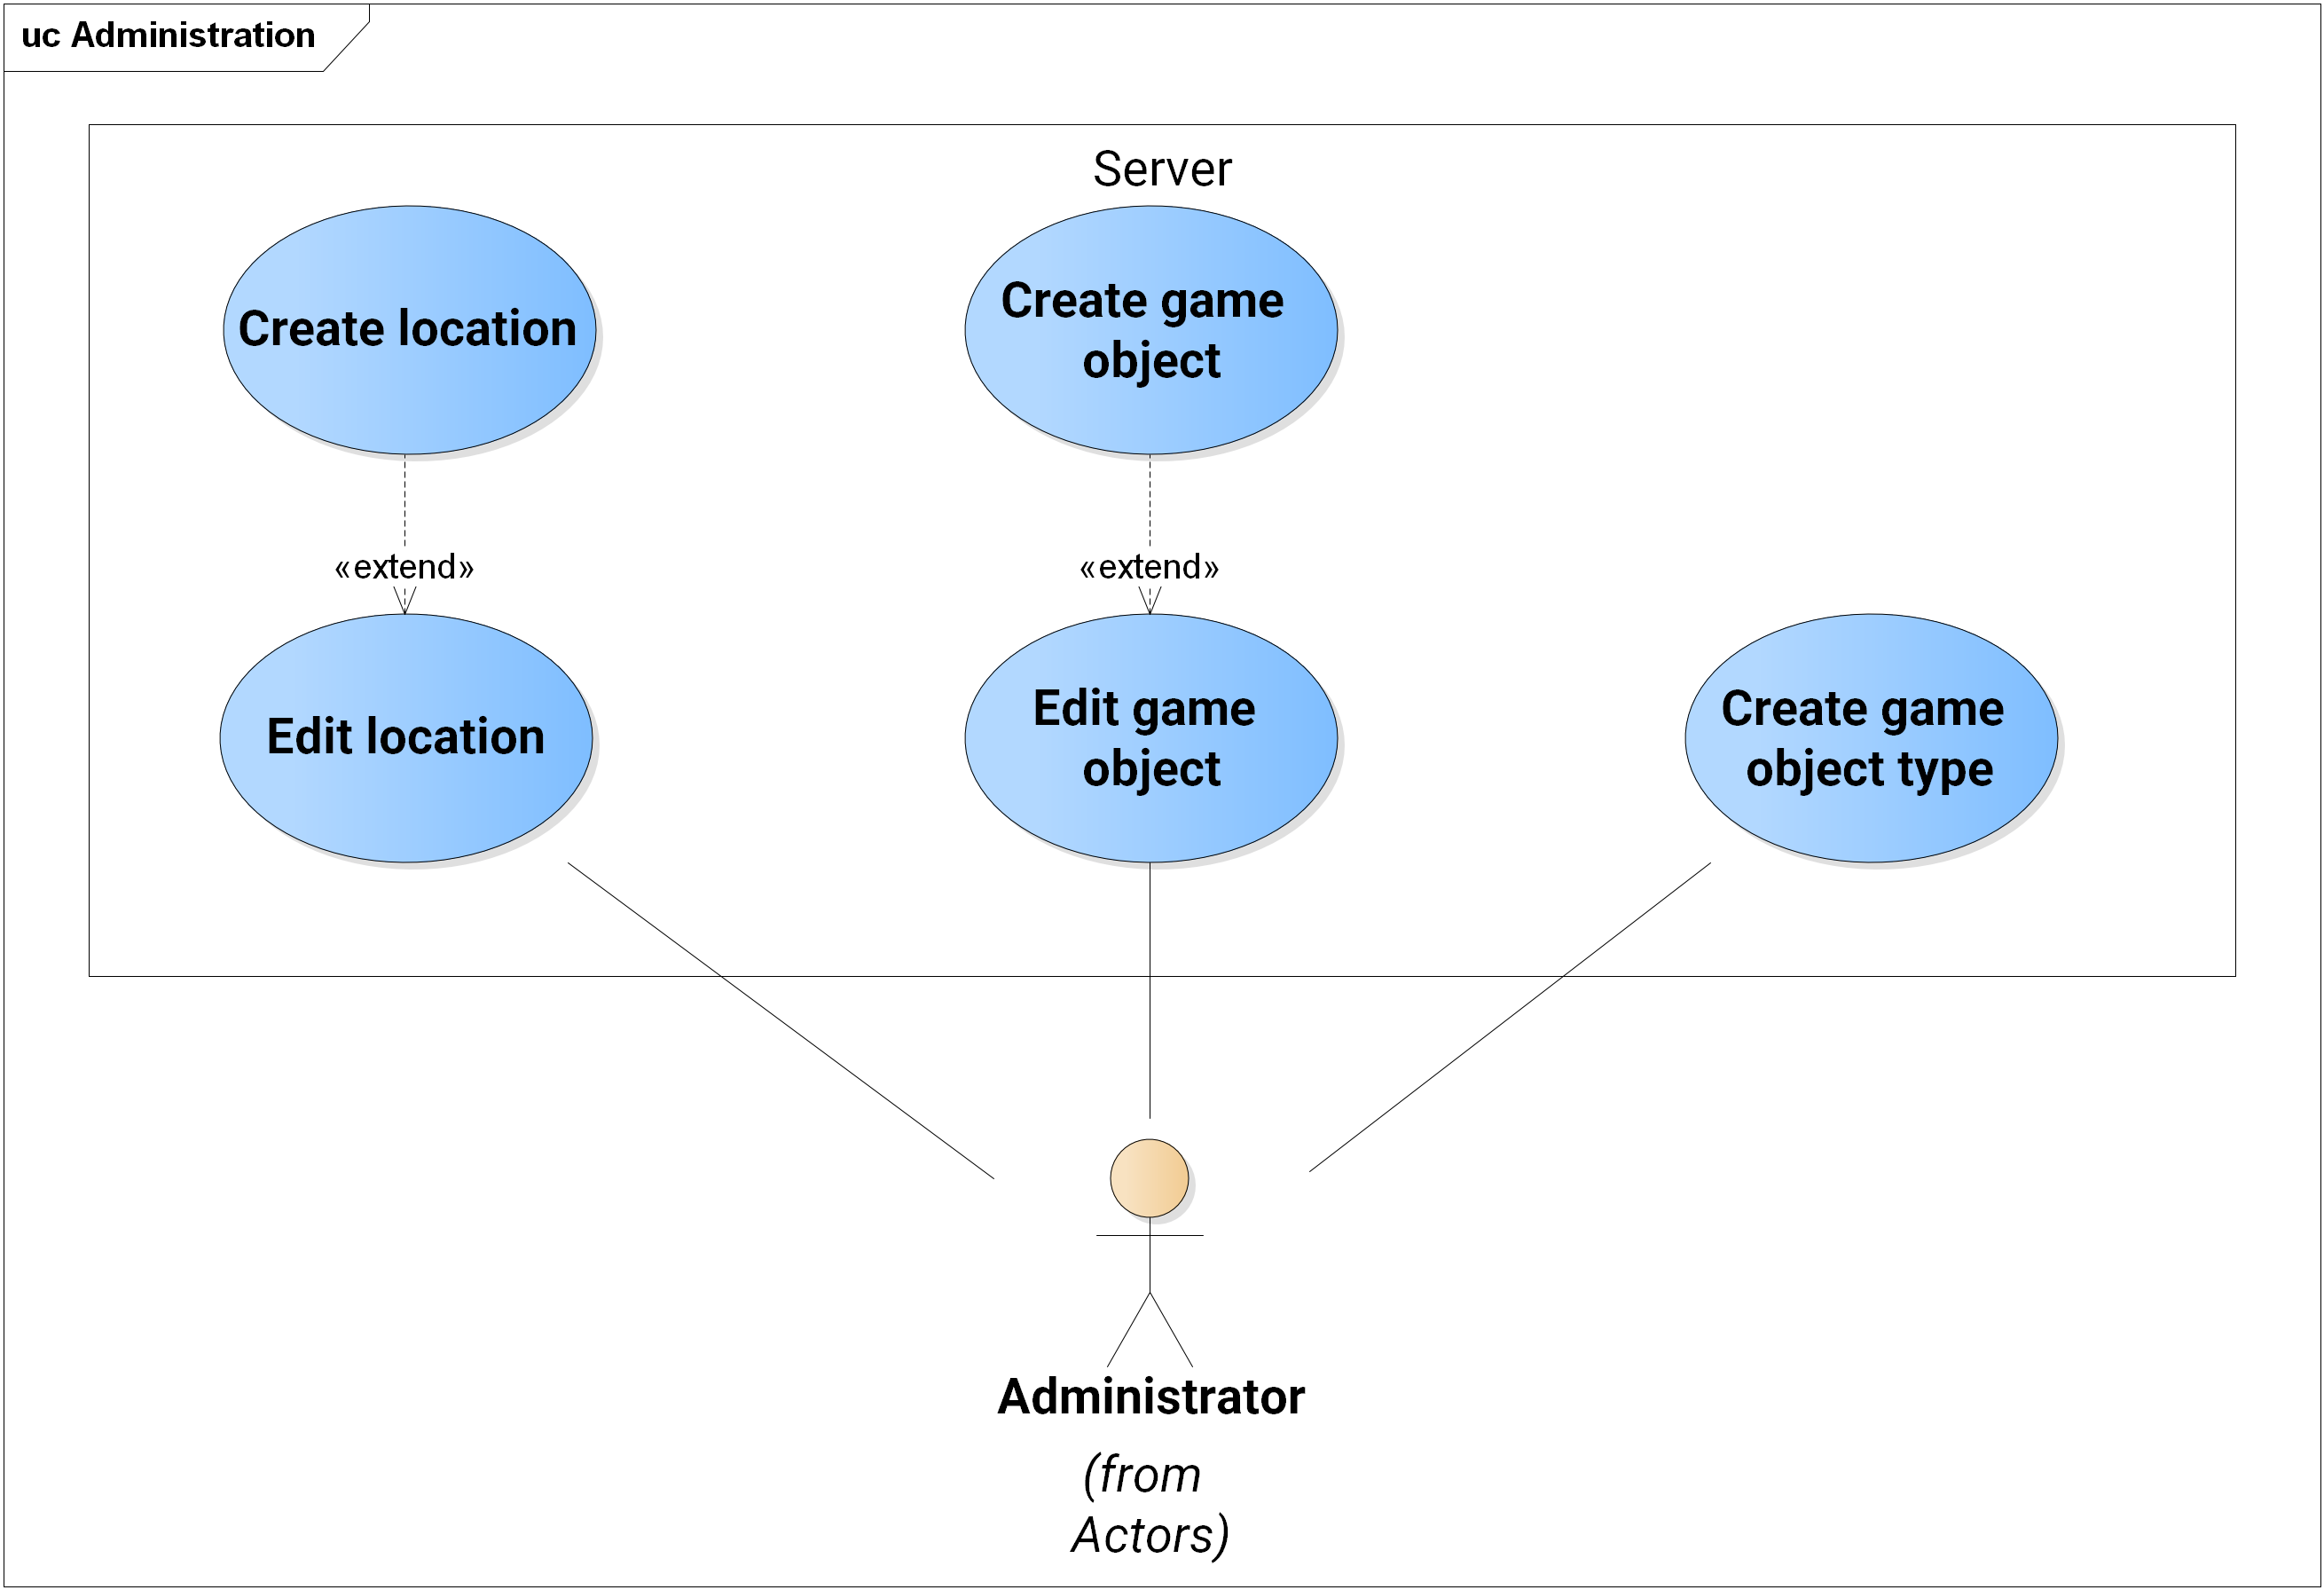
\includegraphics[width=\textwidth]{figures/UC_Administration}
		\centering			
		\caption{Use Cases: Administration}
		\label{fig:ucadmin}				
	\end{figure}	
	\noindent Since the game is not static during its lifetime, people in charge of the changes needs an easy way to add new locations and maintain game objects. These use cases are described in Figure \ref{fig:ucadmin}.
	
	
\section{Requirements}

	\subsection{Functional Requirements}
	These requirements define functions of the server components.
		\subsubsection*{Rules}
		These requirements specify the functionality not directly accessible to clients.
		\begin{enumerate}						
			\item \textbf{The player's character has attributes} \\
			The character has a set of attributes, including health, experience, level, and owned gold. Maximum health increases with level. The experience is rewarded after certain actions, e.g. after killing a monster. The gold is primary in-game currency.
			  
			\item \textbf{A player can own items} \\
			A player has an inventory which can contain various types of items. The item can be for example sword, potion, armor etc.
			
			\item \textbf{A game object has a type and inherits all its properties} \\
			The type of game object specifies allowed actions, its attributes, default name and description.			
			
			\item \textbf{A game object can be a monster} \\
			The monster can be killed but can also inflict damage to the player. It has its own inventory and there's a reward for killing the monster in a form of gold and experience.
			
			\item \textbf{A game object can be a shop} \\
			The shop can contain several items with specified price.  
			
			\item \textbf{A game object can be an item} \\	
			The item can be one of the many objects useful to a player. Examples of the items are health potion, sword, armor, necklace and similar.
			
			\item \textbf{Each game object has its own inventory} \\
			The inventory contains other game objects. Example of this requirement is a monster with a potion and a sword in its inventory; both will be given to the player who kills the monster.  
			
			\item \textbf{The server stores a list of predefined locations} \\	
			Real geographic locations for the game objects are stored on the server to ensure every player has the same location-object pair. 
								
			\item \textbf{A game object can independently exist at many locations} \\
			This requirement aims to help maintain the game objects efficiently by administrators. It allows creating small set of abstract game objects with predefined inventories and other attributes. 
			
			\item \textbf{If a player kills a monster at a location, the monster will be hidden for a period} \\
			To prevent the player from killing the same monster continuously without a need of moving somewhere else, the location should be hidden for a certain period after the kill.						
					
			\item \textbf{The server must persist player’s profile between sessions} \\
			All the player's attributes, his inventory and equipment must be stored between sessions. Player will continue from the state in which he ended.
			
		\end{enumerate}
		\subsubsection*{Features}
		These requirements contain the behavior directly visible to clients.
		\begin{enumerate}
			\item \textbf{The server must provide REST-like API to clients} \\
			The key requirement for the server is to allow receiving HTTP(S) requests. When processed, the server responds in JSON format.
			
			\item \textbf{A player registers and logs in the game using Google account} \\
			For the player's convenience, a Google account is required to play. The server does not have to store or handle any password. Most of the authentication process is delegated to Google servers.
			
			\item \textbf{A client can get nearby game objects based on his location} \\
			The major feature of this application is being location-aware. Server must provide a method to retrieve game locations near the requested latitude and longitude. The "near area" should be circular, defined by its radius; the size have to be carefully chosen so it's big enough to cover client's maps but also small to limit the response size and the spatial search overhead.
			
			\item \textbf{A player can kill a monster} \\
			When the player wins the fight, he will be rewarded by experience and gold. 			
			
			\item \textbf{A player can be killed be a monster} \\
			The player can lose health during the fight with a monster. If the health reaches zero, the player dies and loses an amount of gold based on his level.
			
			\item \textbf{A player can collect items from the monster he killed} \\
			When the player wins the fight, he's offered to collect items from the monster's inventory. He can chose any subset of these items.
			
			\item \textbf{A player can equip an item} \\	
			Many items in the game can be equipped. These items have predefined equipment slot, for example a sword have to be held in hand, an armor worn on chest, shoes put on feet and so on.
						
			\item \textbf{A player can buy object from a shop} \\
			Gold can be exchanged for various items in shops.
			
			\item \textbf{A player can use an item from his inventory} \\
			Some items in the game are consumables. When used, an action defined by the item is executed. For example a health potion heals the player.
			
			\item \textbf{A player can purchase in-app product} \\
			The application allow a user to exchange real-life currency for the in-game one. The server should verify such purchase and add the currency to his profile.
			
			\item \textbf{The server should provide REST-like API for administration} \\	
			Such API will be used to manage locations, create and edit game objects or to assign a game object to some locations. It is necessary to protect the administration endpoints from unauthorized access.
			
		\end{enumerate}
		
		
	\subsection{Non-functional Requirements}
		These requirements specify the criteria the application must meet.
		\begin{enumerate}	
			\item \textbf{Database implements caching} \\
			This application is heavy database reliant. Additional cache provides optimization for faster reads. 				
			
			\item \textbf{The communication between client and server parts of the application must be secure} \\
			All data sent from and to a client has to be encrypted. This should be achieved by connecting to the server via HTTPS.
	
			\item \textbf{The server responsibilities are delegated to its components} \\
			The whole server consists of three components:
			\begin{itemize}
				\item Connection server	(\textit{CS})							
				\item Login server (\textit{LS})
				\item Database server (\textit{DS})
			\end{itemize} 			
			Only the Connection server is accessible to clients.
			
			\item \textbf{The server components are scalable} \\
			Each component can run many instances if itself. These instances are mutually independent.
			
			\item \textbf{The user is authenticated by Google} \\
			A user is authenticated using \textbf{Google Play Games} on the client. The authentication is finished by verifying his ID token using \textbf{Google API Client Library}.	
			
			\item \textbf{The execution environment is Java 8}
								
			\item \textbf{The operating system is Debian 8}\\	
			Thanks to the portability of Java applications, other operating systems may be supported. 													
		\end{enumerate}
	
\section{Technology}
	\subsection{Database Management System}
			
	The database is a crucial part of the server. It handles most of the data persistence. Many commercial and open source solutions exist on market nowadays. In the following text, I will analyze three popular relational database management systems (DBMS) -- MySQL, PostgreSQL, and Oracle. For a quick comparison, see Table \ref{tab:comparedbms}. The described advantages and disadvantages are based on \cite{dbcomparison}.
	\begin{table}
		\centering
		\begin{tabular}{p{0.215\textwidth} || p{0.215\textwidth} | p{0.215\textwidth} | p{0.215\textwidth}}
			& \textbf{MySQL} & \textbf{Oracle} & \textbf{PostgreSQL} \\ 
			\hline \hline
			Rank\footnote{Description of the ranking methodology available at \url{https://db-engines.com/en/ranking_definition}} & 2 & 1 & 4 \\ \hline				
			Initial Release & 1995 & 1980 & 1989 \\ \hline
			License & GPLv2\newline Commercial & Commercial & BSD-like\\ \hline
			Version\footnote{Current stable version as of 2017/06/05} & 5.7 & 12c & 9.6 \\ \hline						
			Replication\newline methods & Master-master\newline Master-slave & Master-master\newline Master-slave & Master-slave  \\ \hline
			SQL Support & yes & yes & yes \\ \hline
			Foreign keys & yes & yes & yes \\ \hline
			JDBC Support & yes & yes & yes \\ \hline
			In-memory\newline capabilities & yes & yes & no \\ \hline				
		\end{tabular}
		\caption{Comparison of popular relational DBMS \cite{dbengines}}
		\label{tab:comparedbms}
	\end{table}	

		\subsubsection{MySQL}
		MySQL \cite{mysql} is an open source relational database management system. It is written mostly in C++ and C \cite{mysqllanguage}.  Currently developed by Oracle, MySQL is available to consumers in several editions. Free Community Edition is released under GPLv2 license\footnote{GPLv2 license text is available at \url{https://www.gnu.org/licenses/gpl-2.0.html}}. Oracle also offers commercial Standard and Enterprise editions which include additional technical support, and monitoring and management tools \cite{mysqleditions}. This DBMS is very widely used and has a strong community base. 
		
		Community Edition includes graphic interface for database management. It also contains a user-friendly modeling tool which allows fast development of the database. The model can be converted to an SQL script and easily deployed on other MySQL servers.
		
		The main advantages: open source, great community support, lightweight, good replication support, powerful management tools.
		
		The main disadvantages: little performance optimization, limited security,  issues with reliability.
		
		\subsubsection{Oracle}
		Oracle Database \cite{oracledb} is an object-relational database management system. Developed by Oracle, it aims on enterprise-scale applications and is well suitable for large businesses. Offered editions include Standard Edition 2 and Enterprise Edition (EE) which can be further expanded by some additional services. The price of EE start at \$950 per user\footnote{Oracle Technology Global Price List, June 1, 2017}. This DBMS is very widely used in corporate environment.
		
		The main advantages: suitable for large databases, well scalable, extensive backup mechanisms.
		The main disadvantages: closed source, free version has very limited feature set, expensive.
		 
		\subsubsection{PostgreSQL}
		PostgreSQL \cite{postgres}, also known as Postgres, is an object-relational database management system. Developed by PostgreSQL Global Development Group, a community of many companies and individuals, PostgreSQL is an open source project licensed under permissive PostgreSQL License \footnote{PostgreSQL License text is available at \url{https://opensource.org/licenses/PostgreSQL}}.
		
		The main advantages: open source, advanced business/location analytics features, good reliability and data-integrity.
		
		The main disadvantages: ill-suited for read-heavy application, poor replication.
				
		\subsubsection{Chosen solution}
		All the presented solutions are similar and are well-supported by Java frameworks. I chose MySQL 5.7 Community Edition to be the database system for this server. I have good experience with MySQL environment and the cost of game development can be lower thanks to the free Community Edition. 
		
	\subsection{Frameworks and Libraries}
	Frameworks provide developer with a powerful tool boc. The tools in this box help in many different areas of application developement. They provide essential design patterns and structure to the development project and also provide the backbone and container for the components to operate within \cite{frameworks}.
	
	I chose to use a Java framework which provide a support for Representational State Transfer (REST) API. Furthermore, I added an Object/Relational Mapping (ORM) framework which helps me to interconnect Java application and MySQL server.
	
		\subsubsection{Dropwizard}
		Dropwizard \cite{dropwizard} glues together many mature libraries which helps with developing a powerful web-application. The libaries most useful for this project include:
		\begin{itemize}
			\item \textbf{Jetty}\\
			Powerful open source web server. Jetty is flexible and extensible. It is a lightweight server with small footprint \cite{jetty}.
			\item \textbf{Jersey}\\
			Jersey RESTful Web Services framework is open source framework for developing RESTful Web Services in Java. It supports JAX-RS\footnote{Specification of JAX-RS is available at \url{https://jcp.org/en/jsr/detail?id=311}} APIs \cite{jersey}.
			\item \textbf{Jackson}\\
			Jackson is a JSON parser and generator. It supports a conversion from JSON to Plain Old Java Object (POJO) and vice versa.			
		\end{itemize}
		\subsubsection{Hibernate ORM}
		Hibernate ORM enables to more easily develop applications whose data outlives the application process. It is an Object/Relational Mapping framework and handles data persistence as it applies to relational database. Hibernate supports many powerful features like lazy initialization and numerous fetching strategies. It requires not special database tables and much of the SQL is generated at system initialization \cite{hibernate}.
		
		\subsubsection{Google API Client Libraries}
		A library developed by Google to help developers integrate Google API to their applications \cite{googleapilibs}. The library is included in this project to handle user authentication and to verify in-app purchases.
		
	\subsection{Index and Cache}
	Redis is an open source in-memory data structure store \cite{redis}. I chose to use Redis as the second level cache provider for Hibernate. The additional cache should result in more optimized database calls and thus performance boost.
	
	Since our application relies heavily on working with geo-spatial data, I decided to implement an additional index. Redis provides a native support for indexing and  searching points near the selected spatial location.		